% You should title the file with a .tex extension (hw1.tex, for example)
\documentclass[a4paper, 12pt]{report}

\usepackage{amsmath}
\usepackage{amssymb}
\usepackage{tabularx}
\usepackage{fancyhdr}
\usepackage{minted}
\usepackage{amsthm}        
\usepackage{graphicx}

\renewcommand\qedsymbol{$\blacksquare$}


\graphicspath{ {./pictures} }

\usepackage[margin=1in]{geometry}

\newcommand{\question}[2] {\vspace{.25in} \hrule\vspace{0.5em}
\noindent{\bf #1: #2} \vspace{0.5em}
\hrule \vspace{.10in}}
\renewcommand{\part}[1] {\vspace{.10in} {\bf (#1)}}

\newcommand{\myname}{Krittin Nisunarat}
\newcommand{\myhwnum}{1}
\newcommand{\mySubject}{ICCS315 Applied Algorithms}

\setlength{\parindent}{20pt}
\setlength{\parskip}{5pt plus 1pt}
 
\pagestyle{fancyplain}
\lhead{\fancyplain{}{\textbf{Project}}}      % Note the different brackets!
\rhead{\fancyplain{}{\myname}}
\chead{\fancyplain{}{\mySubject}}

\title{
	{
\includegraphics[width=80mm,scale=0.5]{MUIC_Logo_Eng_Center.png}} \\
	{\textbf{\mySubject}}\\
	{\large Assignment \myhwnum \ Report}\\
}
\author{
	{\textbf{Written by}} \\ 
	{Krittin Nisunarat 6280782}
}
\date{30 Jan 2022}
\thispagestyle{plain}


\begin{document}
\maketitle
\tableofcontents

\chapter{Resizeable Arrays}

\chapter{Space usage of skip lists}

\chapter{Skip lists}

\chapter{(a,b) tree}

\section{Multiple keys insertion.}

Starting with an empty tree, we want to insert the following keys:
\begin{center}
        733, 703, 608, 846, 309, 269, 55, 745, 548, 449, 513, 210, 795, 656, 262
\end{center}

The result of \emph{(2,3) tree} is

\begin{figure}[h]
        \centering
        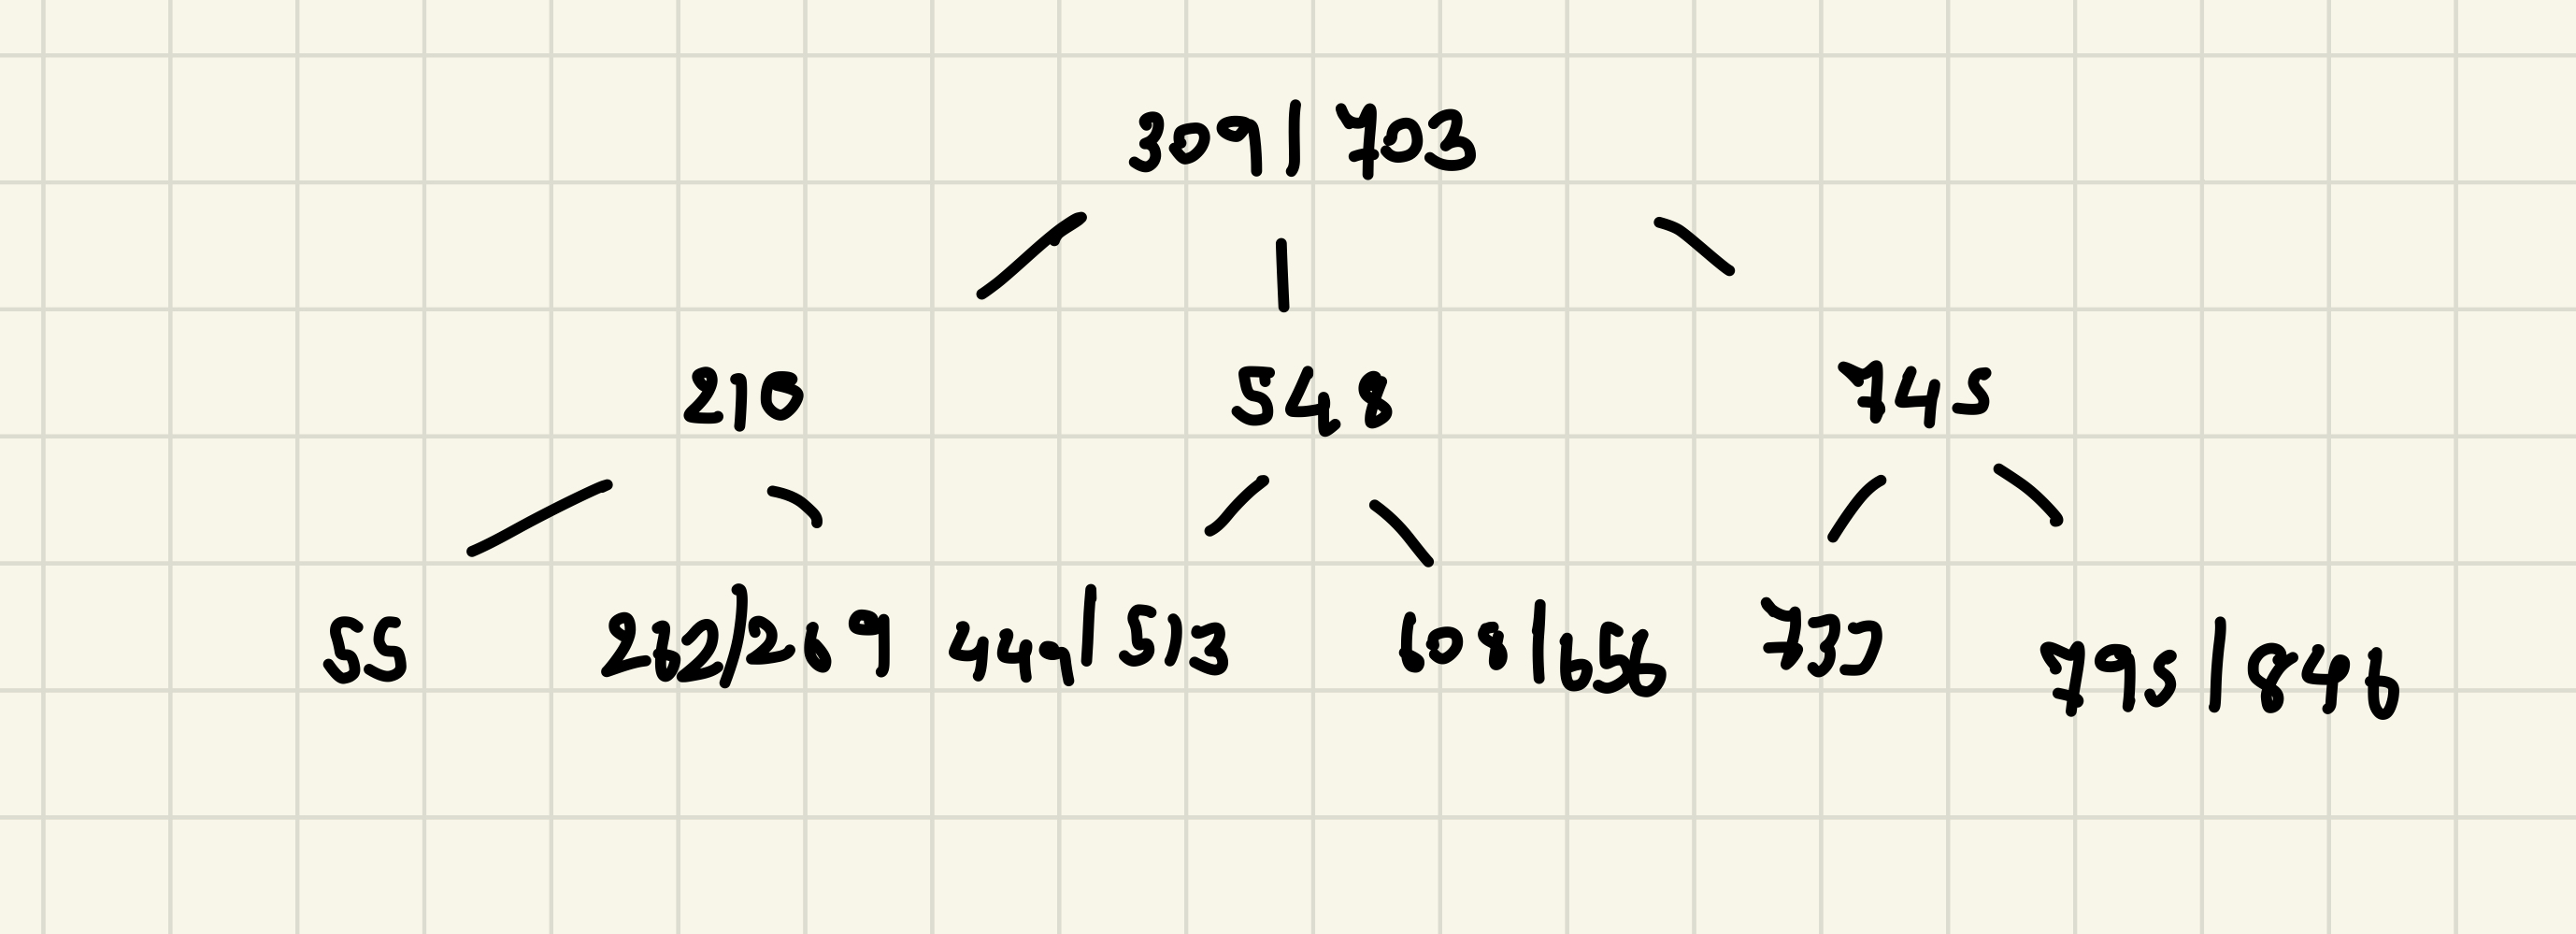
\includegraphics[width=0.9\textwidth,scale=0.5]{tree_insertion.jpeg}
\end{figure}

\section{Key deletion}

\noindent Suppose that we want to delete 309 in \emph{(2,3) tree}, it falls into case 1 which 
we need to steal from sibling.

\begin{figure}[h]
        \centering
        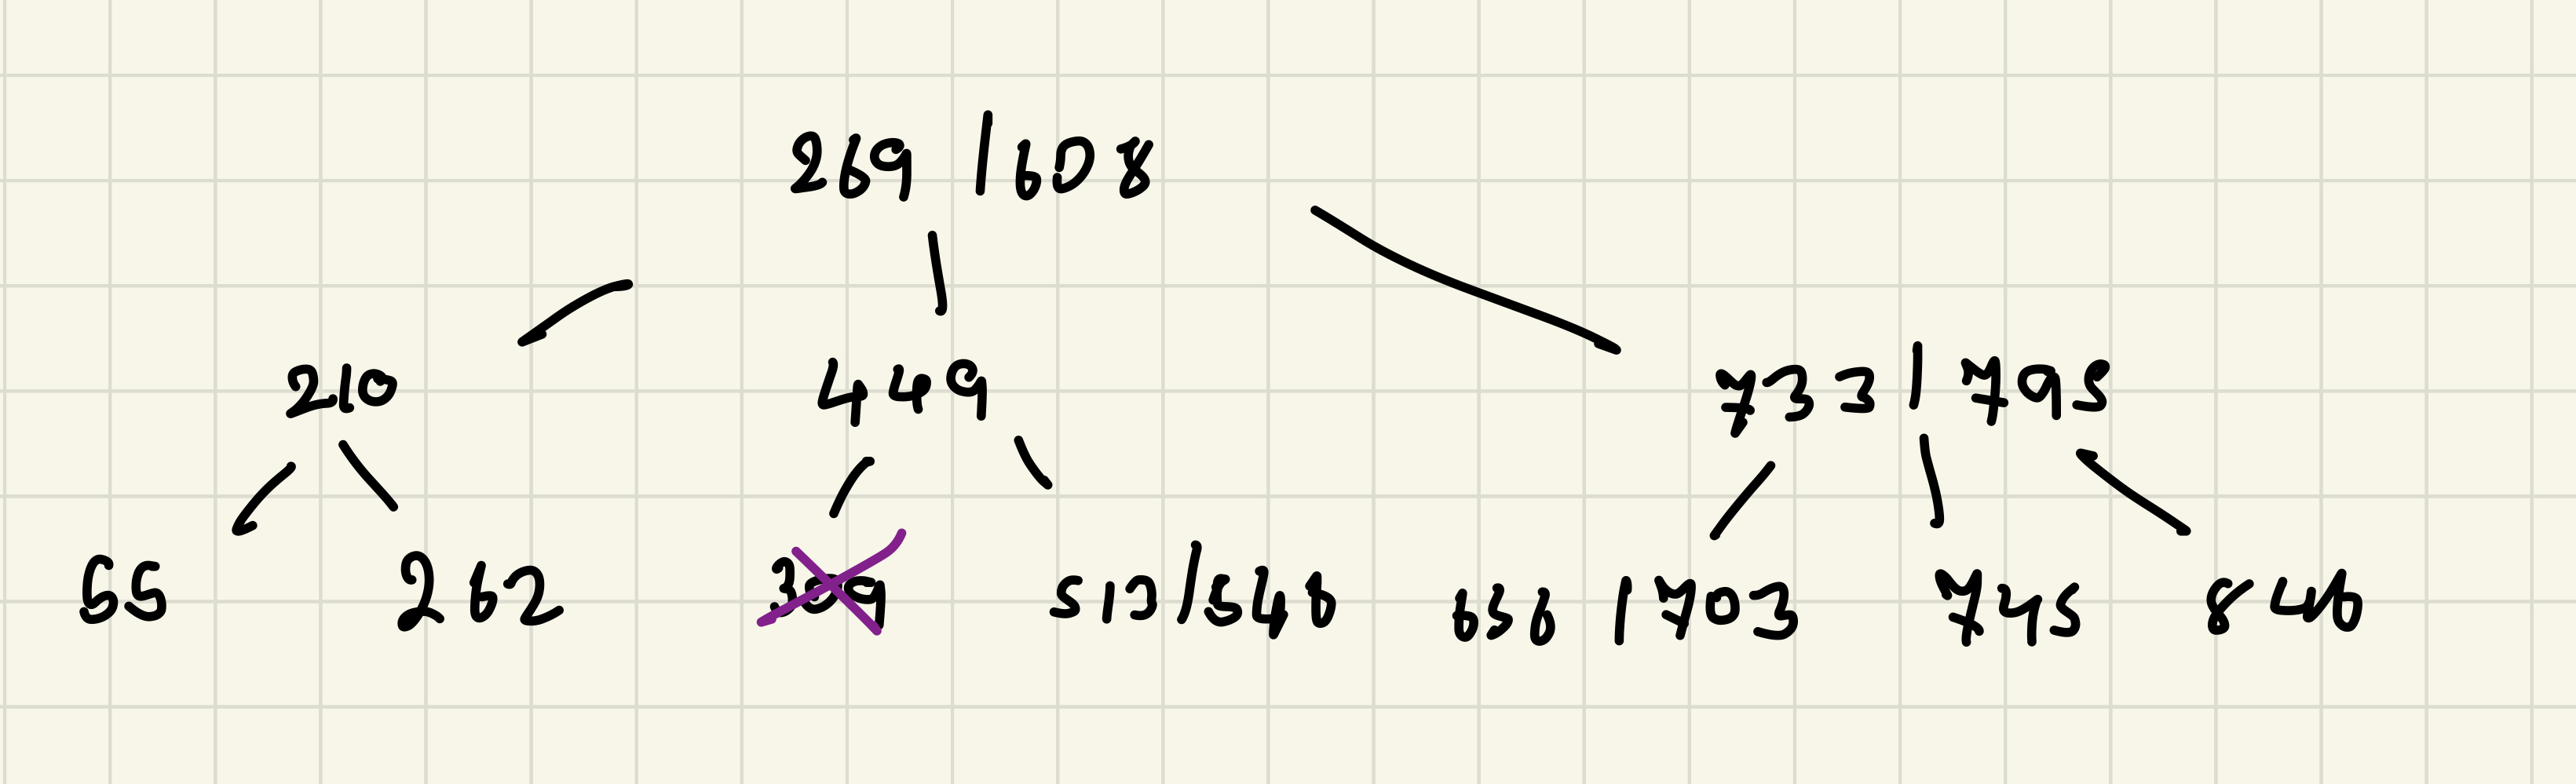
\includegraphics[width=0.8\textwidth,scale=0.5]{tree_deletion_1.jpeg}
        \caption{\label{fig:tree-deletion-1} Unbalanced tree without key 309}
\end{figure}

\begin{figure}[h]
        \centering
        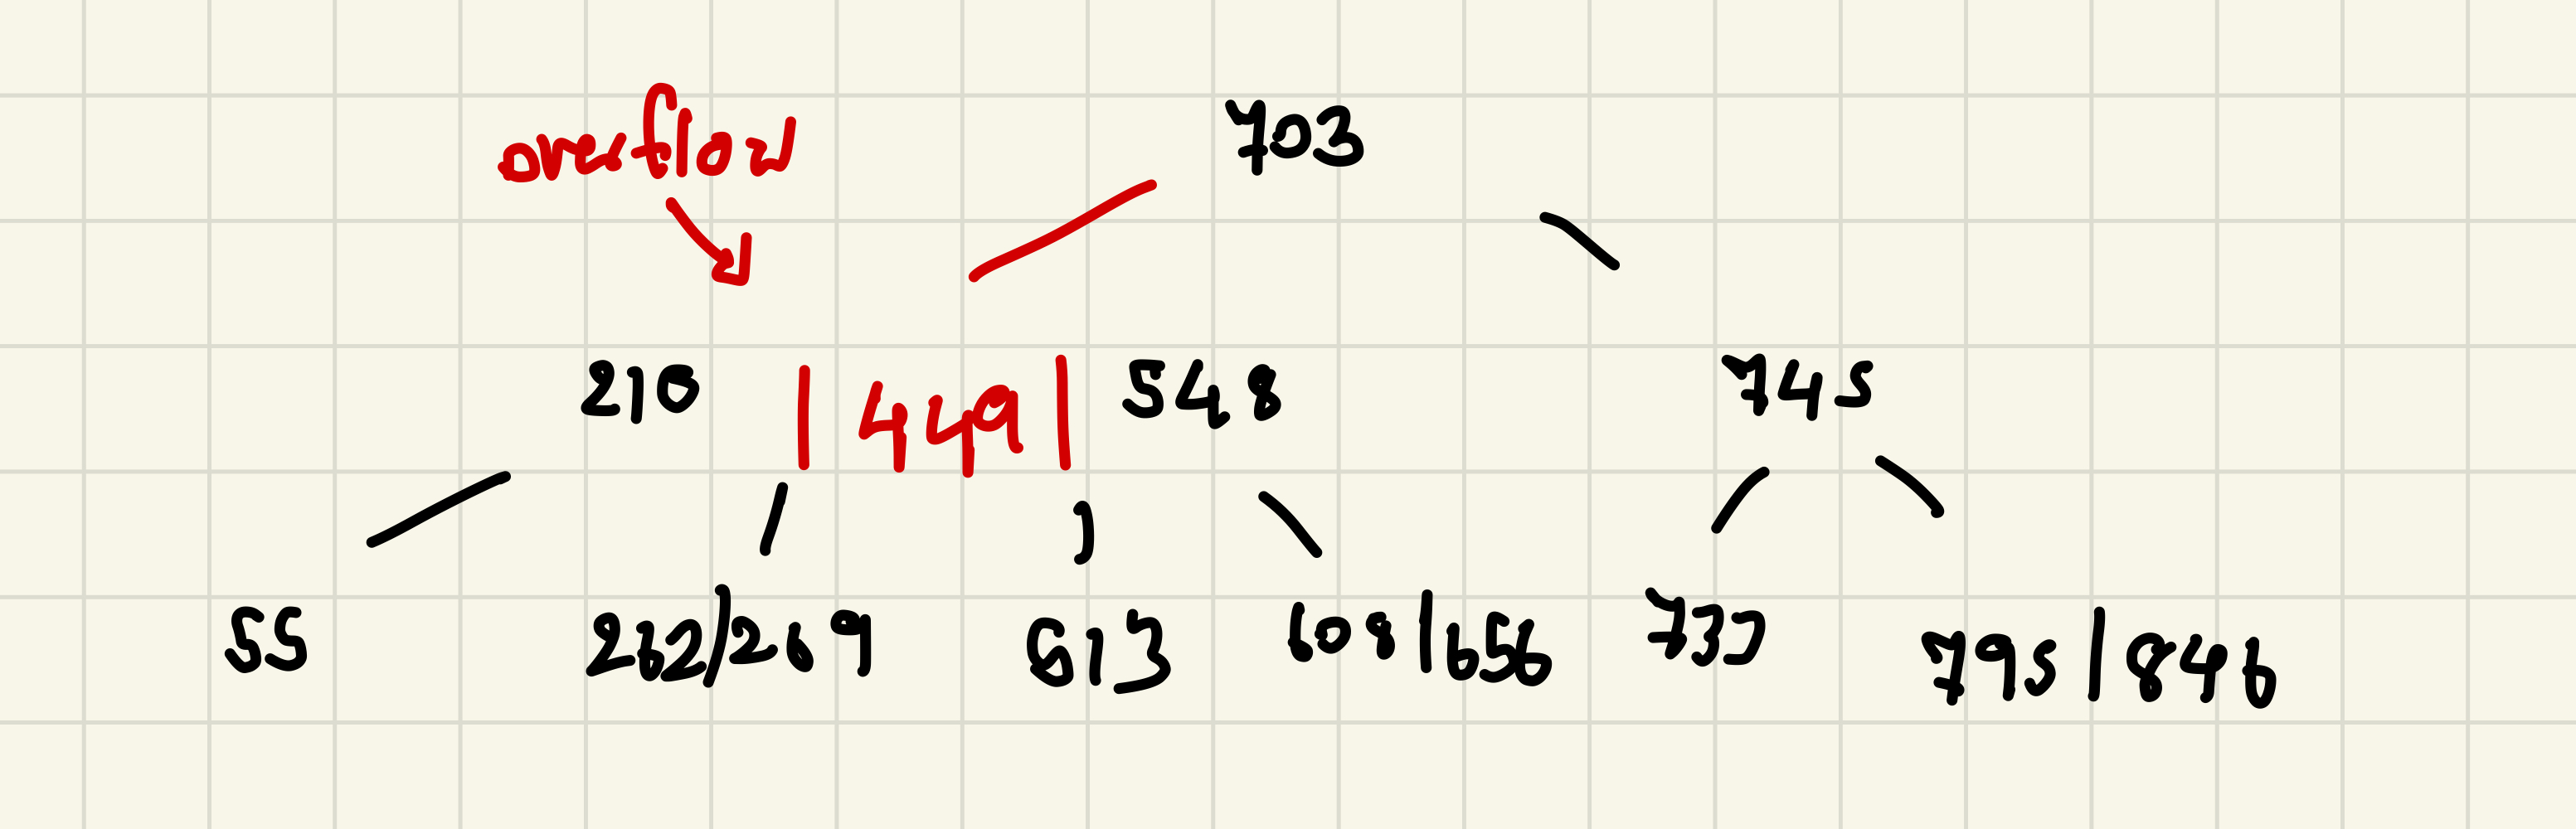
\includegraphics[width=0.8\textwidth,scale=0.5]{tree_deletion_2.jpeg}
        \caption{\label{fig:tree-deletion-2} Balanced tree after finding replacement by stealing}
\end{figure}

As you can see in Figure \ref{fig:tree-deletion-2}, the replacements are 513 and 449 which 513 is the new parent node
that has 449 and 548 as a child nodes. 
\begin{align*}
        \alpha_{\text{me}} = a - 1 + 1
\end{align*} 


\chapter{B-tree speed}
\end{document}
